\documentclass[]{subfiles}

\begin{document}
\section{Projektplanung}
    \subsection{Projektübersicht}
    Das Testen von Netzwerkkonfigurationen findet auch heute noch hauptsächlich 
    mit handgeschriebenen CLI-Befehlen oder kleinen Skripten statt. 
    Wenn der Netzwerktechniker einen Test vergisst, oder die Formulierung nicht stimmt,	
    kann es vorkommen, dass im Netzwerk Fehler auftreten, deren Ursprung schwierig zu 
    ermitteln ist und eine komplette Repetition der (handgeschriebenen) Tests erfordert.

    Ein Programm, welches wie in der Softwareentwicklung vordefinierte und automatisch 
    durchgeführte Tests, sogenannte Unit-Tests, ermöglicht, könnte diese Probleme 
    stark verringern.

    \subsection{Zweck und Ziel}

    Die Studienarbeit soll aufzeigen, dass Studierende unter Anwendung der im Studium erlernten
    Fähigkeiten in der Lage sind, Ingenieurstätigkeiten durchzuführen.
    
    Mit NUTS2.0 soll ein Tool entwickelt werden, welches es Netzwerkleuten erlaubt, 
    Unit Tests in Netzwerkumgebungen durchzuführen. 
    Die Anwendung von Tests erlaubt eine höhere Stabilität und Fehlertoleranz des Systems.

    \subsection{Projektorganisation}
        \subsubsection{Projektmitglieder}
            \begin{tabularx}{0.9\textwidth}{lX}
                \toprule
                Name & Email \\
                \midrule
                Janik Schlatter & \url{jschlatt@hsr.ch} \\
                Mike Schmid & \url{mschmid@hsr.ch} \\
                \bottomrule
            \end{tabularx}

        \subsubsection{Externe Schnittstellen}
            \begin{tabularx}{0.9\textwidth}{lXl}
                \toprule
                Name & Email & Zuständikeit \\
                \midrule
                Beat Stettler & \url{beat.stettler@hsr.ch} & Betreuer \\
                Urs Baumann & \url{urs.baumann@hsr.ch} & Betreuer \\
                \bottomrule
            \end{tabularx}

    \subsection{Managementabläufe}

    \subsubsection{Zeitbudget}
		Das Projekt wurde am 20.02.2020 gestartet und wird voraussichtlich am 28.05.2020 enden.
		Das heisst, es stehen 15 Wochen während dem Semester zur Verfügung. 
        Jedes Projektmitglied arbeitet insgesamt 240 Stunden an dem Projekt, 
        sprich 16 Stunden pro Woche pro Projektmitglied.
        Da der Dienstag 14.04.2020 und der Donnerstag 21.05.2020 jeweils ein Unterrichtsfreier 
        Tag ist, werden die 16 Stunden pro Projektmitglied auf jeweils vier Samstage im Projekt 
        verteilt aufgeteilt.
        Diese Samstage dienen dem Ziel, die Dokumentation nachzutragen und die Risiken, 
        wie sie im Kapitel~\ref{subsec:Risikomanagement} beschrieben sind, zu minimieren. 
        Dazu gehören Bugfixing, Recherchen und Aufarbeiten von Themen, 
        die ungenügend verstanden sind und Refactoring des Codes.

		\begin{table}[!h]
			\begin{tabularx}{\textwidth}{Xl}
				\midrule
				Projektdauer & 15 Wochen \\
				\midrule
				Anzahl Projektmitglieder & 2 \\
				\midrule
				Arbeitsstunden pro Woche und Person & 16 \\
				\midrule
				Arbeitsstunden insgesamt & 480 \\
				\midrule
				Projektstart & 20.02.2020 \\
				\midrule
				Projektende & 28.05.2020 \\
				\midrule
			\end{tabularx}
			\caption{Projektparameter}
        \end{table}
        
    \newpage

	\paragraph{Zeitliche Planung}
        Die 15 Wochen des Projekts werden in fünf Phasen unterteilt: 
        Initialisierung, Analyse, Design, Realisierung und Abschluss.\\
		\begin{figure}[!h]
			\begin{center}
				\label{ZeitplanOverview}
				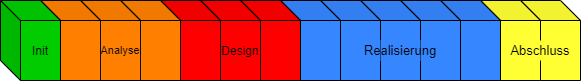
\includegraphics[scale=0.7]{\vorlagenOrdner/Bilder/Projektphasen}
			\end{center}
			\caption{Zeitplanung}
		\end{figure}

    \subsubsection{Projektphasen}
		\begin{table}[!h]
			\begin{tabularx}{\textwidth}{lll}
				\toprule
				Farbe & Bezeichnung & Zeitrahmen \\
				\midrule
				\textcolor{green}{Grün} & Initialisierung & 1 Woche \\
				\textcolor{orange}{Orange} & Analyse & 3 Wochen \\
				\textcolor{red}{Rot} & Design & 3 Wochen \\
				\textcolor{blue}{Blau} & Realisierung & 6 Wochen \\
				\textcolor{yellow}{Gelb} & Abschluss & 2 Wochen \\
				\bottomrule
			\end{tabularx}
			\caption{Projektphasen}
		\end{table}

    \subsubsection{Meilensteine}
    \begin{table}[!h]	
        \begin{tabularx}{\linewidth}{lllX}
            \toprule
            Nr & Bezeichnung & Termin & Beschreibung \\
            \midrule
            M1 & Projektplan & So 01.03.2020 & Grundentwurf der Requirements, Risikoanalyse \& -management, Projektorganisation, Managementabläufe, Infrastrukturentwurf, Qualitätsmassnahmen Grundentwurf.\\
            \midrule
            M2 & Requirements & So 15.03.2020 & Ausgearbeitete Requirements, Nichtfunktionale Anforderung, Zu verwendende Tools und Schnittstellen beschrieben.\\
            \midrule 
            M3 & Prototyp & So 05.04.2020 & Architektur festgelegt, Schnittstellen angelegt, Architekturdokumentation, Erster lauffähiger Prototyp.\\
            \midrule
            M4 & Feature Freeze & Do 07.05.2020 & Hauptfunktionalität der Software implementiert, Bugs sind bekannt und Dokumentiert, Codedokumentation zu 60\% fertiggestellt.\\
            \midrule
            M5 & Codefreeze & So 24.05.2020 & Bugfixes erstellt, Tests sind alle erfolgreich, Codedokumentation zu 80\% fertiggestellt.\\
            \midrule
            M6 & Projektabgabe & Do 28.05.2020 & Dokumentation fertiggestellt und abgegeben.\\
            \bottomrule
        \end{tabularx}
    \caption{Meilensteine}
    \end{table}	

    \subsubsection{Iterationen}
    \begin{table}[!h]
        \begin{tabularx}{\textwidth}{lXll}
            \toprule
            Iteration & Inhalt & Start & Ende \\
            \midrule
            Initialisierung & Projektstart und Kick-Off Meeting & 20.02.2020 & 23.02.2020 \\
            \midrule
            Analyse 1 & Projektplanung & 24.02.2020 & 01.03.2020 \\
            Analyse 2 & Evaluation Module (Nornir, Napalm, Openconfig) & 02.03.2020 & 08.03.2020 \\
            Analyse 3 & Requirements \& Analyse Testcases & 09.03.2020 & 15.03.2020 \\
            \midrule
            Design 1 & Architekturdesign & 16.03.2020 & 22.03.2020 \\
            Design 2 & Testen der Module & 23.03.2020 & 29.03.2020 \\
            Design 3 & Prototyp programmieren & 30.03.2020 & 05.04.2020 \\
            \midrule
            Realisierung 1 & Umsetzung Filehandler, Testrunner,  & 06.04.2020 & 12.04.2020 \\
             & Inventarmanagement und Testdefinitionsklassen & & \\
            Realisierung 2 & Umsetzung Testerstellung-Strategy-Factory & 13.04.2020 & 19.04.2020 \\
             & und Testresultat-Mapper & & \\
            Realisierung 3 & Umsetzung Connection-Strategy-Factory und Evaluator & 20.04.2020 & 26.04.2020 \\
            Realisierung 4 & Umsetzung Testbuilder, Testcontroller, und Reporter & 27.04.2020 & 03.05.2020 \\
            Realisierung 5 & Umsetzung Testreihenfolge, automatische  & 04.05.2020 & 10.05.2020 \\
             & Geräteerfassung und Kommandozeilen-UI & & \\
            Realisierung 6 & Fertigstellung und Refactoring & 11.05.2020 & 24.05.2020 \\
            \midrule
            Abschluss 1 & Bugfixes, Refactoring und Dokumentation & 18.05.2020 & 24.05.2020\\
            Abschluss 2 & Fertigstellung Schlussbericht & 23.05.2020 & 28.04.2020\\
            \bottomrule
        \end{tabularx}
        \caption{Projektiterationen}
    \end{table}

    \subsubsection{Arbeitspakete}
    Die Arbeitspakete sind in vier Kategorien eingeteilt, um eine Übersicht zu bieten. 
    \begin{itemize}
        \item Ausführung der Tests - Alles was mit der Ausführung und Evaluation der Netzwerktests zu tun hat.
        \item Erstellen der Tests - Alle Arbeitspakete, die sich mit der Erstellung der Testsuite auseinandersetzen.
        \item Hilfsklassen - Filehandler, Logging, Integration Tests und Kommandozeileninteraktion
        \item Tests - Integration einzelner Tests in das System
    \end{itemize}
    
        \minisec{Kategorie Ausführung der Tests}       
        \paragraph*{Implementation Testrunner}\mbox{} \\
        \begin{tabularx}{\textwidth}{lX}
            \toprule
            Beschreibung & Die Testrunner-Klasse führt die ihm vom Controller übergebenen Tests gegen das Netzwerk aus und gibt ein Resultat in einem beliebigen Format zurück.\\
            \midrule
            Akzeptanzkriterien & Testrunner ist in der Lage, Tests gegen ein Netzwerk auszuführen und reagiert auf Fehler, indem fehlgeschlagene Tests als solche annotiert werden.\\
            \midrule
            Aufwandschätzung & 6 Stunden\\
            Tatsächlicher Aufwand & 4 Stunden \\
            \midrule
            Priorität & Mittel \\
            \bottomrule
        \end{tabularx}
    
        \paragraph*{Implementation Evaluator}\mbox{} \\
        \begin{tabularx}{\textwidth}{lX}
            \toprule
            Beschreibung & Der Evaluator vergleicht die Resultate der Netzwerktests mit den aus den Testdefinitionen beschriebenen Soll-Werten.\\
            \midrule
            Akzeptanzkriterien & Der Evaluator ist in der Lage, die normalisierten Testresultate mit den Testexpectations zu vergleichen und ein verständliches Evaluationsresultat zu erzeugen.\\
            \midrule
            Aufwandschätzung & 10 Stunden\\
            Tatsächlicher Aufwand & 6 Stunden\\
            \midrule
            Priorität & Mittel \\
            \bottomrule
        \end{tabularx}
        \newpage
    
        \paragraph*{Implementation Reporter}\mbox{} \\
        \begin{tabularx}{\textwidth}{lX}
            \toprule
            Beschreibung & Der Reporter nimmt die Gesamtergebnisse entgegen und gibt sie auf der Konsole in einem einfach verständlichen Format aus. \\
            & Zudem schreibt er die Ergebnisse in ein Report-File, welches die Testresultate und allfällige Fehlermeldungen beinhaltet. \\
            \midrule
            Akzeptanzkriterien & Die Reporter-Klasse ist in der Lage, detaillierte Berichte zu den Ergebnissen zu verfassen und abzuspeichern.\\
            \midrule
            Aufwandschätzung & 10 Stunden\\
            Tatsächlicher Aufwand & 12 Stunden\\
            \midrule
            Priorität & Niedrig \\
            \bottomrule
        \end{tabularx}
    
        \paragraph*{Implementation Testresultat-Mapper}\mbox{} \\
        \begin{tabularx}{\textwidth}{lX}
            \toprule
            Beschreibung & Der Testresultatmapper normalisiert die Rückgabewerte der einzelnen Netzwerktests in ein einheitliches Format, so dass der Evaluator damit arbeiten kann.\\
            \midrule
            Akzeptanzkriterien & Die Normalform der Resultate ist festgelegt und implementiert.\\
            \midrule
            Aufwandschätzung & 12 Stunden\\
            Tatsächlicher Aufwand & 11 Stunden \\
            \midrule
            Priorität & Mittel \\
            \bottomrule
        \end{tabularx}
    
        \paragraph*{Implementation Testcontroller}\mbox{} \\
        \begin{tabularx}{\textwidth}{lX}
            \toprule
            Beschreibung & Der Testcontroller ist der Einstiegspunkt in das Programm. Er instanziert die benötigten Klassen und steuert den Programmfluss.\\
            \midrule
            Akzeptanzkriterien & Testcontroller ist implementiert und das Programm lässt sich erfolgreich ausführen.\\
            \midrule
            Aufwandschätzung & 4 Stunden \\
            Tatsächlicher Aufwand & 10 Stunden \\
            \midrule
            Priorität & Niedrig \\
            \bottomrule
        \end{tabularx}
        \newpage
    
        \minisec{Kategorie Erstellen der Tests}
    
        \paragraph*{Implementation Testbuilder}\mbox{} \\
        \begin{tabularx}{\textwidth}{lX}
            \toprule
            Beschreibung & Der Testbuilder übernimmt die Tests aus der Testdefinition und erstellt ein Testbundle mit den angegebenen Parameter. \\
            \midrule
            Akzeptanzkriterien & Der Testbuilder ist implementiert und erstellt ausführbare Tests.\\
            \midrule
            Aufwandschätzung & 6 Stunden\\
            Tatsächlicher Aufwand & 12 Stunden\\
            \midrule
            Priorität & Mittel\\
            \bottomrule
        \end{tabularx}
    
        \paragraph*{Auswahl der Testreihenfolge}\mbox{} \\
        \begin{tabularx}{\textwidth}{lX}
            \toprule
            Beschreibung & Erweiterung des Testbuilder um die Möglichkeit, die Reihenfolge der Tests zu bestimmen.\\
            \midrule
            Akzeptanzkriterien & Testdurchführungsreihenfolge lässt sich ändern.\\
            \midrule
            Aufwandschätzung & 6 Stunden\\
            Tatsächlicher Aufwand & 18 Stunden \\
            \midrule
            Priorität & Niedrig\\
            \bottomrule
        \end{tabularx}
    
        \paragraph*{Inventar Management Klassen}\mbox{} \\
        \begin{tabularx}{\textwidth}{lX}
            \toprule
            Beschreibung & Zu diesem Arbeitspaket gehören die Klassen Inventar, Device und DeviceConnection. Diese Klassen beschäftigen sich damit, die Informationen über die Physischen Geräte in einem Netzwerk festzuhalten.\\
            \midrule
            Akzeptanzkriterien & Klassen sind implementiert und die Zusammenarbeit funktioniert. Es lassen sich Tests mit den Gerätedaten vom TestBuilder erstellen und durchführen.\\
            \midrule
            Aufwandschätzung & 10 Stunden\\
            Tatsächlicher Aufwand & 14 Stunden\\
            \midrule
            Priorität & Hoch \\
            \bottomrule
        \end{tabularx}
        \newpage
    
        \paragraph*{Testdefinition Klassen}\mbox{} \\
        \begin{tabularx}{\textwidth}{lX}
            \toprule
            Beschreibung & Die Testdefinitionen beschreiben die auszuführenden Tests gegen das Netzwerk. Der Loader instanziert die Definitionen der einzelnen Tests und gibt diese als Collection an den Testbuilder weiter, der daraus konkrete Tests instanziert.\\
            \midrule
            Akzeptanzkriterien & Testdefinitionen lassen sich erstellen und ausführen.\\
            \midrule
            Aufwandschätzung & 8 Stunden\\
            Tatsächlicher Aufwand & 10 Stunden\\
            \midrule
            Priorität & Hoch\\
            \bottomrule
        \end{tabularx}
    
        \paragraph*{Connection-Strategy-Factory}\mbox{} \\
        \begin{tabularx}{\textwidth}{lX}
            \toprule
            Beschreibung & Dieser Teil der Software kümmert sich um die Auswahl und Instanzierung der Kommunikationsschnittstelle.\\
            \midrule
            Akzeptanzkriterien & Alle Klassen sind gemäss der Architektur implementieren und es lässt sich mindestens eine Schnittstelle auswählen und instanzieren.\\
            \midrule
            Aufwandschätzung & 20 Stunden\\
            Tatsächlicher Aufwand & 5 Stunden\\ 
            \midrule
            Priorität & Hoch\\
            \bottomrule
        \end{tabularx}
    
        \paragraph*{Testerstellung-Strategy-Factory}\mbox{} \\
        \begin{tabularx}{\textwidth}{lX}
            \toprule
            Beschreibung & Dieser Teil des Programms entscheidet, welche konkreten Testklassen verwendet werden und instanziert diese.\\
            \midrule
            Akzeptanzkriterien & Alle Klassen sind gemäss der Architektur implementiert und es gibt mindestens eine konkrete Testklasse die sich ausführen lässt. \\
            \midrule
            Aufwandschätzung & 20 Stunden\\
            Tatsächlicher Aufwand & 24 Stunden\\ 
            \midrule
            Priorität & Hoch\\
            \bottomrule
        \end{tabularx}
        \newpage
    
        \paragraph*{Automatische Geräteerfassung}\mbox{} \\
        \begin{tabularx}{\textwidth}{lX}
            \toprule
            Beschreibung & Damit das Inventar nicht von Hand geführt werden muss, lassen sich die Geräteeinstellungen automatisch erfassen.\\
            \midrule
            Akzeptanzkriterien & Die Erfassung lässt sich erfolgreich durchführen, sie erfasst sämtliche Geräte im Netzwerksystem und speichert die Daten im YAML-Format.\\
            \midrule
            Aufwandschätzung & 30 Stunden\\
            Tatsächlicher Aufwand & 0 Stunden (Wurde nicht Implementiert)\\ 
            \midrule
            Priorität & Niedrig\\
            \bottomrule
        \end{tabularx}
        \newpage
    
        \minisec{Kategorie Hilfsklassen}
    
        \paragraph*{FileHandler}\mbox{} \\
        \begin{tabularx}{\textwidth}{lX}
            \toprule
            Beschreibung & Der Filehandler wird immer dann aufgerufen, wenn etwas aus dem Filesystem geladen werden muss oder etwas darin geschrieben werden soll.\\
            \midrule
            Akzeptanzkriterien & Der Filehandler ist implementiert und es lassen sich damit Dokumente im YAML Format schreiben und lesen.\\
            \midrule
            Aufwandschätzung & 6 Stunden\\
            Tatsächlicher Aufwand & 10 Stunden\\ 
            \midrule
            Priorität & Hoch\\
            \bottomrule
        \end{tabularx}
    
        \paragraph*{Logging}\mbox{} \\
        \begin{tabularx}{\textwidth}{lX}
            \toprule
            Beschreibung & Der Logger ist dafür zuständig, dass alle Events, die in der Software geschehen, beispielsweise Exceptions oder Informations-Logs, persistent gespeichert werden.\\
            \midrule
            Akzeptanzkriterien & Der Logger ist implementiert.\\
            \midrule
            Aufwandschätzung & 6 Stunden\\
            Tatsächlicher Aufwand & 5 Stunden\\ 
            \midrule
            Priorität & Niedrig\\
            \bottomrule
        \end{tabularx}
    
        \paragraph*{Integration Tests}\mbox{} \\
        \begin{tabularx}{\textwidth}{lX}
            \toprule
            Beschreibung & Mit den Integration Tests wird überprüft, ob die Softwarekomponenten alle miteinander zusammen agieren können. Sie dienen der Überprüfung des Systems.\\
            \midrule
            Akzeptanzkriterien & Integrationstests wurden systematisch und geplant durchgeführt und die Resultate dokumentiert. Allfällige Fehler wurden im Issue-Tracking erfasst.\\
            \midrule
            Aufwandschätzung & 10 Stunden\\
            Tatsächlicher Aufwand & 5 Stunden\\ 
            \midrule
            Priorität & Niedrig\\
            \bottomrule
        \end{tabularx}
        
        \paragraph*{Kommandozeilen-UI}\mbox{} \\
        \begin{tabularx}{\textwidth}{lX}
            \toprule
            Beschreibung & Um mit dem Programm interagieren zu können, wird ein Grafikinterface benötigt.\\
             & Vorerst wird dieses mit einem Kommandozeilen-Userinterface umgesetzt.\\
            \midrule
            Akzeptanzkriterien & Es ist möglich, die Erfassung, Orchestrierung und Durchführung über die Kommandozeile zu steuern.\\
            \midrule
            Aufwandschätzung & 14 Stunden\\
            Tatsächlicher Aufwand & 8 Stunden\\ 
            \midrule
            Priorität & Mittel \\
            \bottomrule
        \end{tabularx}
        \newpage
    
        
    
        \minisec{Kategorie Test-Integration}
        Die Testintegration befasst sich mit der Implementation der einzelnen Netzwerktests. 
        Für die meisten Tests sollte ein Aufwand von vier bis acht Stunden ausreichend sein, wobei umfangreichere Tests durchaus mehr Zeit für die Implementation benötigen können.
        Die Integration von weiteren Tests hat geringe Priorität, solange die Kernfunktionalität des Programms noch nicht fertiggestellt ist. 
        Ausnahme dafür ist der Ping-Test, welcher für die Entwicklung zum Ausprobieren verwendet wird und ein bis drei weitere Tests, welche für das Integration-Testing verwendet werden.
    
        Mögliche Tests:
        \begin{itemize}
            \item ping
            \item tracert
            \item show ip interface 
            \item show ip protocols
            \item show ip route
            \item show interfaces
            \item iperf
            \item nmap portscan
            \item show ip ospf interface
            \item show ip ospf neighbor
            \item show ip eigrp neighbors
            \item show ip bgp 
            \item show ip route bgp 
            \item show ip bgp neighbors
            \item show mpls lsp extensive
            \item show mpls neighbor
            \item show isis adjacency
            \item show isis interface
        \end{itemize}

    \subsection{Risikomanagement}
    \label{subsec:Risikomanagement}

    \subsubsection{Risikoanalyse}
    \minisec{Risiken zu Beginn der Studienarbeit}
    \begin{figure}[!h]
        \begin{center}
            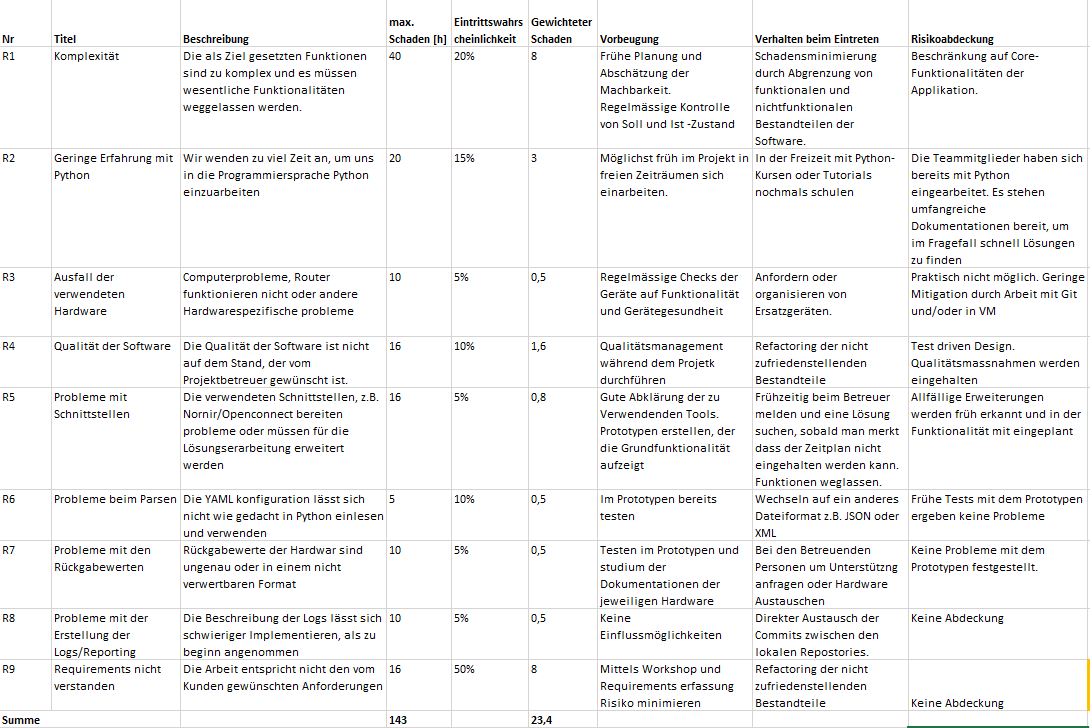
\includegraphics[scale=0.6]{\vorlagenOrdner/Bilder/Risikoanalyse1}
        \end{center}
        \caption{Risikoanalyse zu Beginn der Arbeit}
    \end{figure}

    \newpage

    \minisec{Angepasste Risiken am Ende der Studienarbeit}
    \begin{figure}[!h]
        \begin{center}
            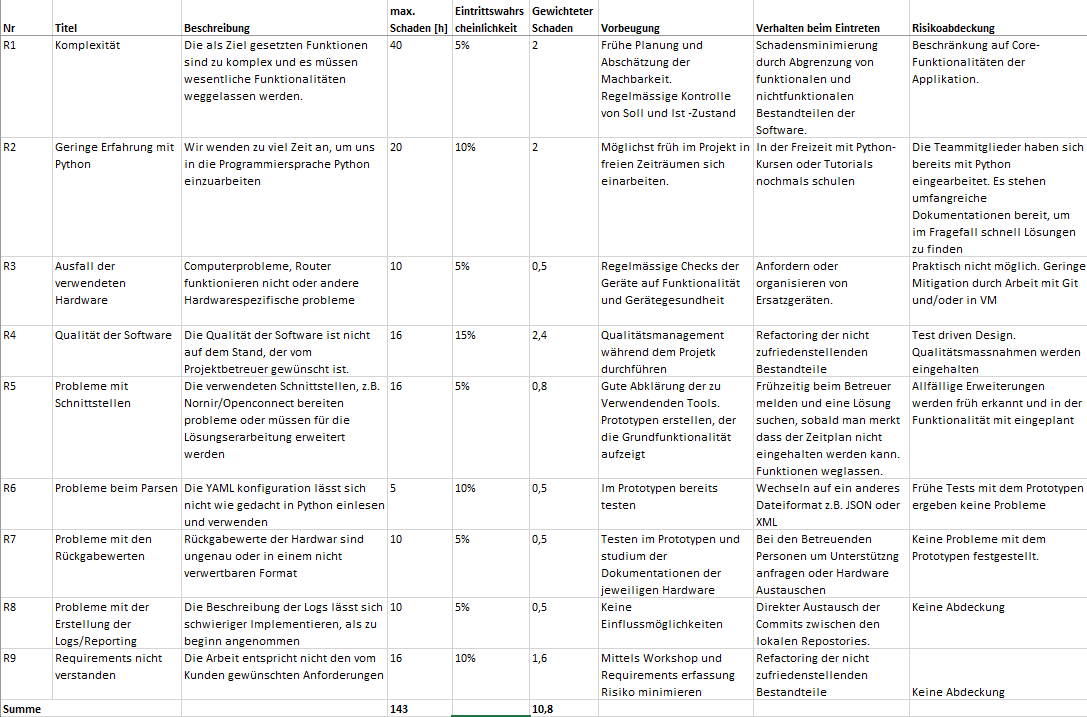
\includegraphics[scale=0.6]{\vorlagenOrdner/Bilder/Risikoanalyse2}
        \end{center}
        \caption{Angepasste Risiken am Ende der Studienarbeit}
    \end{figure}

    \subsubsection{Umgang mit Risiken}
    Um Probleme gerade während der Init/Analyse Phase möglichst früh zu erkennen, 
	arbeiten wir wöchentlich zwei Tage nebeneinander, um uns über mögliche Probleme auszutauschen. 
	Des Weiteren suchen wir auch den Kontakt zum Betreuer sobald Unklarheiten im Team herrschen.
    Einmal alle zwei Wochen sind  am Samstag für drei bis vier Stunden vorgesehen,
    um an der Dokumentation und and der Reduktion aufgetretener Risiken zu arbeiten. 
    
    Darüber hinaus ist in der Zeitplanung keine Reserve für Risiken eingeplant und die 
    Projektmitglieder werden im Eintretensfall zusätzliche Arbeit verrichten müssen, 
    um die verlorene Zeit aufzuholen.


\end{document}